\chapter{Zeitplanung}
Die Umsetzung der Masterarbeit ist in einem Zeitrahmen von sechs Monaten geplant. Ein Gantt-Diagramm, das die Tätigkeiten, deren Zeitbedarf und die terminliche Planung visualisiert, wird in Abb. \ref{fig:gantt} dargestellt.
Die Tätigkeiten, die in diesem Diagramm dargestellt werden, wurden aus Kapitel \ref{cha:concept} über die Konzeption übernommen und werden hier nicht mehr detailliert beschrieben. Es folgt lediglich eine Erläuterung des Zeitbedarfs.

Für den ersten Teil, in welchem die \gls{gui} entwickelt wird, werden 12 Wochen veranschlagt. Zu Beginn steht dabei ein größerer Evaluationsteil, in dem die verschiedenen Frameworks evaluiert und eventuell an die Nutzung angepasst werden. Anschließend folgen verschiedene konsekutive Implementierungsarbeiten. Die Aufteilung bzgl. der Entwicklung der prozeduralen Generierung und der Python-Bindings ist hierbei noch flexibel und hängt davon ab, in welche Programmiersprache die prozedurale Generierung entwickelt wird. Sollte diese in Rust erfolgen, so ist deren Entwicklung komplexer, während die Python-Bindings weniger Zeit benötigen. Im Fall einer Entwicklung in Python ist dies entsprechend umgekehrt.

Der zweite Teil der Arbeit, in dem die Autoencoder entwickelt werden, soll 10 Wochen lang sein und überlappt sich zeitlich etwas mit dem ersten Teil. In dieser Zeitspanne kann eine Einarbeitung in PyTorch erfolgen. Anschließend erfolgen mehrere sich überlappende Tätigkeiten in denen die Autoencoder entwickelt werden. Die Überlappung kommt dadurch zustande, dass hier Feedbackschleifen stattfinden müssen. So sollen die Autoencoder nach der Durchführung von Experimenten erneut angepasst werden um erneut Experimente auszuführen und die Ergebnisqualität zu verbessern. Daher sind diese Tätigkeiten als parallel anzusehen.

Nach den praktischen Tätigkeiten erfolgt noch ein Pufferzeitraum. Bei einigen Tätigkeiten existieren Risiken, die in Kapitel \ref{sec:risks} beschrieben werden. Durch diese Unsicherheiten kann es passieren, dass einige Tätigkeiten mehr Zeit benötigen, als eingeplant wurde, wodurch sich die Arbeit verzögern kann. Sollte dieser Puffer nicht benötigt werden, können weitere Verbesserungen der Autoencoder-Architektur oder Untersuchungen bzgl. der Generalisierbarkeit der Lösung für allgemeine \glspl{gui}, nicht nur für JADX, durchgeführt werden.

Das Schreiben der Masterarbeit ist eine Tätigkeit, die über die gesamte Bearbeitungszeit parallel zu allen anderen Tätigkeiten erfolgen soll. Zum Schluss sind 4 Wochen Zeit eingeplant, in denen der Feinschliff erfolgt, d.h. in denen formale und gestalterische Aspekte sowie Rechtschreibung und Grammatik optimiert werden, fehlende oder unvollständige Teile ergänzt und darüber hinaus die inhaltliche Abstimmung innerhalb der Arbeit verbessert werden sollen.

% \begin{itemize}
%     \item Rust-GUI - 2,5 Monate?
% \begin{enumerate}
%     \item Einarbeitung in Rust
%     \item Auswahl des GUI-Frameworks - 4 Wochen (zusammen mit erstem)
%     \item Entwicklung der GUIs - 3 Wochen? --> wie viele Elemente sind das denn?
%     \item Prozedurale Generierung der GUI - 2 Woche?
%     \item Implementierung der Python-Bindings - 2 Wochen?
%     \begin{itemize}
%         \item Flexibel: Wenn Generierung in Rust, dann mehr Zeit für Generierung und weniger für Python-Bindings. Wenn Generierung in Python, dann weniger Zeit für Generierung und mehr für Python-Bindings
%     \end{itemize}
% \end{enumerate}
% \item Autoencoder - 2 Monate?
% \begin{enumerate}
%     \item Einarbeitung in PyTorch - 2 Wochen
%     \item Entwicklung mehrerer Autoencoder-Architekturen
%     \item Training der Autoencoder
%     \item Experimente mit Autoencodern
% \end{enumerate}
% \item Thesis
% \begin{enumerate}
%     \item Grobe Erstellung - 5 Monate
%     \item Feinschliff - 1 Monat
% \end{enumerate}
% \end{itemize}

\begin{figure}[htbp]
    \centering
    \begin{ganttchart}[
        x unit=0.4cm,
        y unit title=1cm,
        y unit chart=0.8cm,
        vgrid={*{28}{dotted}}
        ]{1}{28}
        \gantttitle{2021}{28} \\
        \gantttitlelist{24,26,...,50}{2} \\
        \ganttgroup{GUI}{1}{12} \\
        \ganttbar{Einarbeitung Rust}{1}{4} \\
        \ganttbar{Auswahl Framework}{1}{4} \\
        \ganttlinkedbar{Impl. GUI}{5}{8} \\
        \ganttlinkedbar{Impl. Generierung}{9}{10} \\
        \ganttlinkedbar{Impl. Python-Bindings}{11}{12} \\
        \ganttgroup{Autoencoder}{11}{20} \\
        \ganttbar{Einarbeitung PyTorch}{11}{13} \\
        \ganttlinkedbar{Entw. Autoencoder}{14}{18} \\
        \ganttbar{Training Autoencoder}{15}{18} \\
        \ganttbar{Evaluierung}{17}{20} \\
        \ganttgroup{Puffer}{21}{24} \\
        \ganttbar{Verschiedenes}{21}{24} \\
        \ganttgroup{Erstellung Thesis}{1}{27} \\
        \ganttbar{Grobe Erstellung}{1}{23} \\
        \ganttlinkedbar{Feinschliff}{24}{27} \\
    \end{ganttchart}
    \caption{Gantt-Diagramm über die Zeitplanung der Bearbeitung in Kalenderwochen}
    \label{fig:gantt}
\end{figure}

% \begin{figure}[htbp]
%     \centering
%     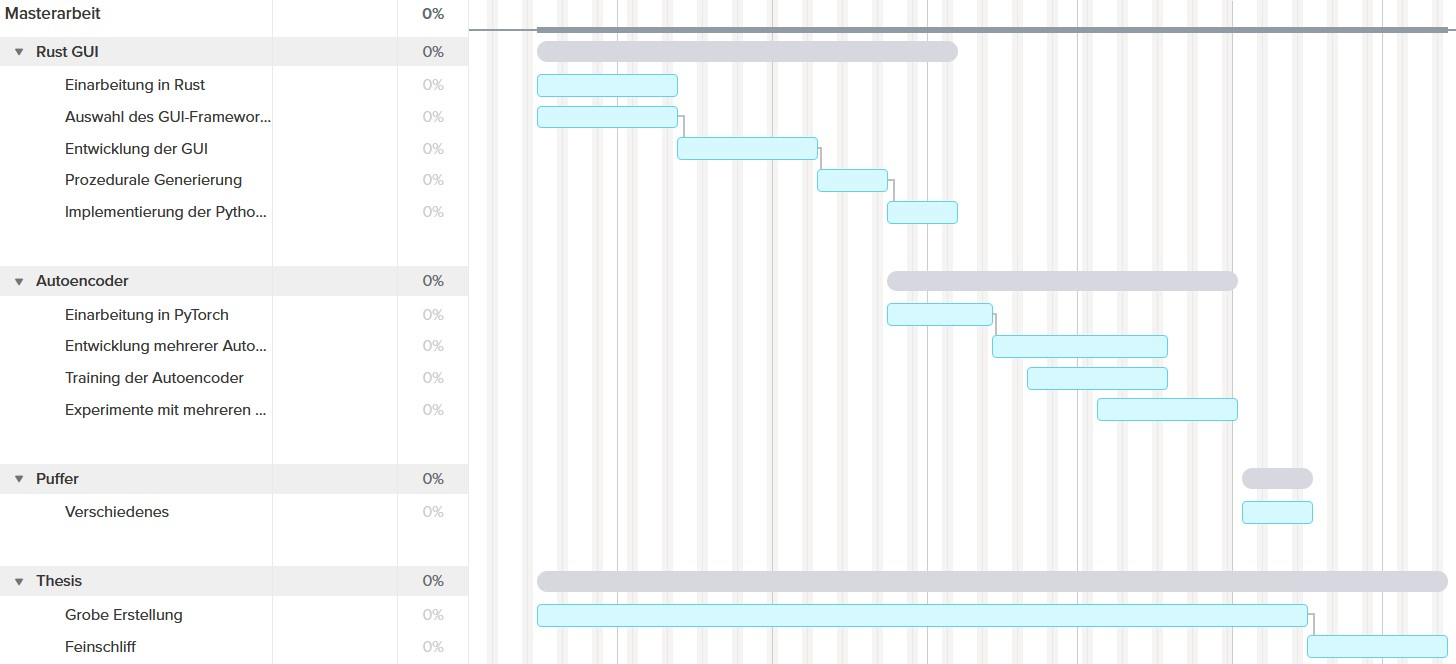
\includegraphics[width=\textwidth]{bilder/ganttChart}
%     \caption{Gantt-Diagramm über die Zeitplanung der Bearbeitung}
% \end{figure}

\chapter{Ausblick}
Im Rahmen der Masterarbeit gibt es aufgrund des großen Evaluierungs- und Implementierungsteils nur begrenzt Zeit das genannte Problem vollumfänglich zu lösen. Daher existieren schon jetzt Fragestellungen, die voraussichtlich erst in späteren Arbeiten gelöst werden können.

Die erste Fragestellung ist, inwiefern die trainierten Autoencoder auch auf allgemeinen \gls{gui}-Oberflächen gut funktionieren. Die geschriebene \gls{gui}-Oberfläche ist an das Programm JADX angelehnt. Für allgemeine Programme, deren Darstellung stark von JADX abweicht müssen deshalb unter Umständen eigene Mock-Oberflächen geschrieben bzw. die hier implementierte Oberfläche weiter generalisiert werden. Eine 1-zu-1-Übertragbarkeit der aus dieser Masterarbeit gewonnenen Erkenntnisse über die Eignung von Autoencodern für die Lösung der Problematik muss ebenso erneut evaluiert werden.